\documentclass{llncs}
\usepackage{amssymb}
\usepackage{url}
\usepackage{graphicx}

\hyphenation{pro-po-si-tion-ali-zation}

\title{Mutlirelatonal GUHA Method and Genetic Data}
\author{Martin Ralbovsk\'{y}, Alexander Kuzmin, Jan Rauch}
\institute{Department of Information and Knowledge Engineering,\\
University of Economics, Prague, W. Churchill Sq.~4, 130 67 Praha~3, Czech Republic\\
\email{martin.ralbovsky@gmail.com, alexander.kuzmin@gmail.com, rauch@vse.cz}}

\begin{document}
\maketitle

\begin{abstract}
The paper presents multirelational GUHA method, focusing on multirelational association rules. Background and principles of the method are introduced together with comparison with related methods. New implementation in the Ferda tool is presented and initial experiments in the genetic domain are shown. 
\end{abstract}

{\small {\bf Keywords:} GUHA method, Multirelational GUHA, 4FT, virtual attribute, Ferda, genetic data}

\section{Introduction}
\label{section:introduction}
The GUHA method is one of the first methods of exploratory data analysis, which has been in development since the mid-sixties. It is a general mainframe for retrieving interesting knowledge from data. The method has firm theoretical foundations based on logics, especially observational calculi and statistics \cite{GUHA2}. Figure \ref{fig:GUHA} shows the main principle of the method. 

\begin{figure}[ht]
\centering
\mbox{\resizebox{50mm}{!}{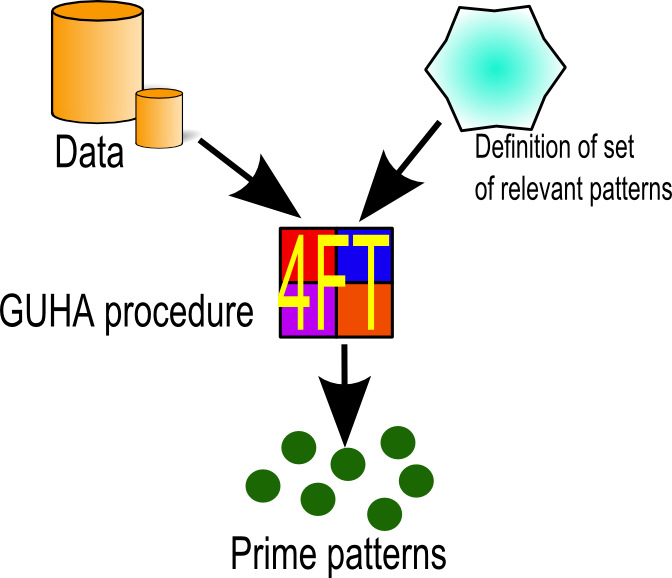
\includegraphics{GUHA.png}}}
\caption{The GUHA method}
\label{fig:GUHA}
\end{figure}

GUHA method is realized by GUHA procedures such as the 4FT procedure, located in the middle of the figure. A GUHA task consists of data and a simple definition of a possibly large set of relevant patterns defined with the aid of observational calculi, which are inputs to the procedure. The procedure automatically generates all the relevant patterns and verifies them against the provided data. Patterns that are true and do not logically follow from the other true output and more simple patterns are called {\em prime patterns}. We call them also {\em hypotheses} as in \cite{GUHA2}. The most known GUHA procedure is the ASSOC (\emph{4ft-miner}, 4FT) procedure for mining generalized association rules \cite{Alternative,Ralbovsky}, based on different approach than the mainstream \emph{apriori} algorithm \cite{Agrawal2}. 

In its initial form, procedures of the GUHA method were designed to mine over one relation only. In \cite{Rauch3}, proper theory for the multirelational form of the method was developed. However, until recently this form lacked suitable implementation and data to prove usability. We present in this paper recent implementation of the multirelational GUHA in the Ferda system \cite{Ferda} and we also start experiments with genetic data where the method seems to be perspective.

The paper is structured as follows: section \ref{section:principles} explains main principles of multirelational GUHA
and briefly introduces the new implementation of the method. Section \ref{section:related} compares our method to other mainly ILP methods and section \ref{section:genetic} describes the initial experiments with genetic data. Finally section \ref{section:conclusion} concludes the paper. 

\section{Principles of Multirelational Mining with GUHA}
\label{section:principles}
Because of the short format of the paper, we explain only basics of the principles without going into detail. For more details, 
see \cite{Rauch3,Karban}. The multirelational GUHA method currently supports star-scheme of the database with one \emph{master table} and several \emph{detail tables}. The key term is \emph{virtual attribute}, which is attribute from detail data table, that is created during the process of GUHA pattern verification and is treated as normal attribute of master table although not physically stored. The most interesting type of virtual attribute is the \emph{hypotheses attribute}. Hypotheses attribute is defined by the GUHA (sub)task on the detail table. Value of the attribute corresponds to validity of a GUHA pattern for subset of records of the detail table that "belongs" to the master record. Validity can be expressed as boolean value or (in the future) generally as a real number. One GUHA (sub)task in on the detail table usually generates large amount of hypotheses attributes. 

\begin{figure}[ht]
\centering
\mbox{\resizebox{80mm}{!}{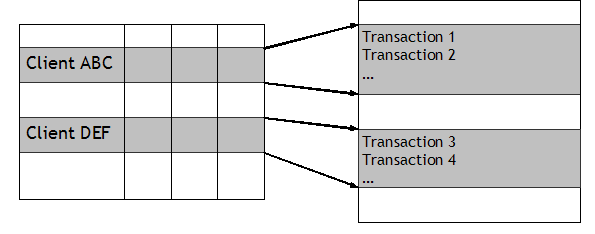
\includegraphics{Transactions.png}}}
\caption{Example of multirelational task setting}
\label{fig:transactions}
\end{figure}

We present an example of the hypotheses attribute from the banking domain\footnote{We think that banking domain is more comprehensible than the genetic domain to the non-expert.}. The used GUHA procedure is 4FT for association rules mining: there are two tables concerning clients of a bank. The master table contains information about clients' accounts and the detail table contains information about transactions of individual clients. One client in the master table can have several transactions in the detail table. Example of hypotheses attribute can be \emph{client that often pays by credit card}, which can be formally written as $$ClientID \approx Payment(CreditCard).$$ The situation is shown in figure \ref{fig:transactions}.
It is obvious, that this rule may be very useful as an attribute in the master table concerning clients' accounts. We name the virtual attribute $ClientPayingByCreditCard.$ Then one can examine status of a client based on client's payments and address. Example of such generalized association rule is
$$District(SouthEast) \& ClientPayingByCreditCard$$
$$\approx Status(good).$$

There are two experimental implementation of relational GUHA method, one in the frame of LISp-Miner system \cite{Alternative} and the second one in the Rel-Miner system \cite{Karban}, but they are not used any more due to various reasons. The new implementation in the Ferda system \cite{Ferda} takes advantage of visual and modular environment, which makes the complex task setting comprehensible to the user. Figure \ref{fig:Ferda} shows a sample multirelational task in Ferda. All the implementations of relational GUHA do not use \emph{apriori}, they are based on representation of  analyzed  data by strings of bits \cite{Alternative}. 

\begin{figure}[ht]
\centering
\mbox{\resizebox{120mm}{!}{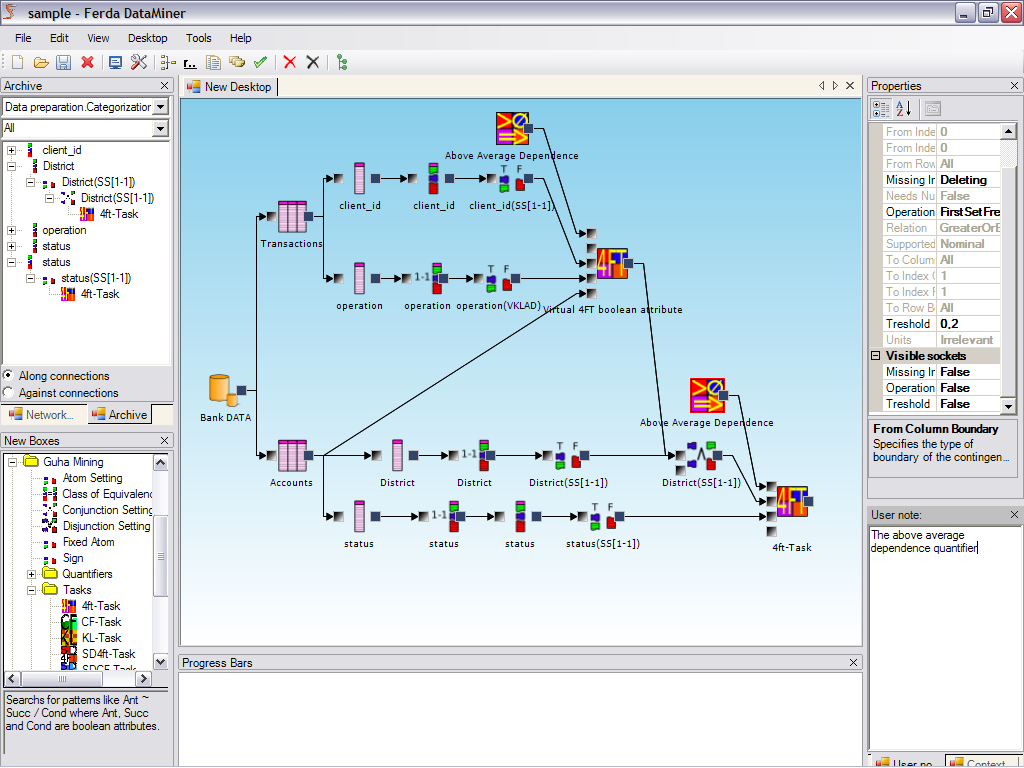
\includegraphics{Ferda.png}}}
\caption{The Ferda environment}
\label{fig:Ferda}
\end{figure}

\section{Related Methods}
\label{section:related}
The most known KDD technique for discovering knowledge from multirelational data is inductive logic programming (ILP). Principle of propositionalization approaches in ILP \cite{ILP} is very close to principle of hypotheses attribute. Below is list of main differences:

\begin{itemize}
	\item Propositioned attributes of ILP are conjunctions of (possibly negated) literals of predicate logic. In contrary, hypotheses attributes are formulas of observational calculus, enabling to represent i.e. implication or statistical significance of the attribute.
	\item In practical cases, multirelational GUHA is limited to star-scheme of the database. Relations in ILP does not have this restriction. 
\end{itemize}

The \emph{WARMR} algorithm \cite{Warmr} performs ILP propositionalization and then searches for association rules in \emph{apriori}-like manner. Detailed comparison of \emph{WARMR} and multirelational GUHA can be found in \cite{Karban}. Another approach based on \emph{apriori} \cite{Connection} adapts \emph{support} and \emph{confidence} measures and calculates them on multiple tables without joining them. The RELAGGS system
\cite{RELAGGS} works in similar manner: it calculates aggregations of records of columns from tables bound by foreign keys. Because the method is based on database joins, it is not unable to calculate the expressive GUHA patterns on the detail tables. 

\section{Mining over Genetic Data}
\label{section:genetic}
The big problem throughout the history of multirelational GUHA was to find suitable domain to prove the usefulness of the method. The first attempts were made in the banking domain - dataset Barbora was used\footnote{Used in the PKDD 1999 Discovery challenge, see \url{http://lisp.vse.cz/challenge}.}. These attempts were unsuccessful.

During this spring, we initiated cooperation with Czech Technical University (CTU) concerning mining genetic data. Team from CTU lead by F. Zelezny compiled genetic dataset from publicly available datasets. The dataset contains genetic measurements acquired from Affymetrix DNA microarrays\footnote{National Center for Biotechnology Information GEO Datasets \url{http://www.ncbi.nlm.nih.gov}} from human, mouse and rat for two different types of cells: hematopoetic and stromal, both of which are involved in blood cells production in bone marrow. The gene measurements were enriched with gene semantics involving information about pathways (maps representing molecular interaction and reaction networks) and fully-coupled-fluxes (FCF), linear pathway subgraphs\footnote{Taken from KEGG genome database, \url{http://www.genome.jp.kegg}}. 

The longterm scientific goal is to examine how does the expression of genes in FCF correlate with types of cells (and possibly other characteristics) \cite{Genes}. Because the expressiveness of hypotheses attribute, multirelational GUHA is especially fit for this purpose. We have tried initial experiments with hypotheses attributes such as \emph{high expression of genes in FCF} showing promising results: one of the experiments included examination of 500K gene measurements concerning 500 FCF's. With procedure 4FT we obtained 1394 \emph{hypotheses} out of 3187 verifications. All the hypotheses were in form:

$$[FluxID(\alpha)\approx_{1} GeneLevel(\beta)] \approx_{1} CellType(\gamma)$$ 

Where $\approx_{1}$ stands for $Conf=100\%$. However following work need to be done in order to obtain scientifically sound results:

\begin{itemize}
	\item \bfseries Proper discretization: \normalfont GUHA has ways to handle numeric data. Yet these ways are unsuitable mainly because of the fact that expressions of different genes have different ranges, but are contained in one attribute. We need to build a new genome expression table based on discrete values directly from Affymetrics DNA microarrays. 
	\item \bfseries Scaling: \normalfont It is the first time that multirational GUHA has been used with data of such a large size and we have experienced performance problems. Effective ways to handle results of queries, which by far exceed the capacity of operating memory need to by found and implemented. 
	\item \bfseries Chip handling: \normalfont The probes measuring one gene are placed on several chips. It remains an open question how much does this fact influence the gene measurement. 
\end{itemize}

\section{Conclusion}
\label{section:conclusion}
We present multirelational extension of the GUHA method of exploratory analysis. Like other methods such as ILP propositionalization, the principle is to enrich a data table with attributes taken from other data tables. The advantage of multirelational GUHA lies in providing an expressive language for virtual attributes based on observational calculus. 

We also present recent implementation of multirelational GUHA method in the Ferda system and possible and promising usage of the method in genetic experiments. At present, we do not yet have any scientifically sound genetic results, the paper states next steps to be made in order to achieve them. Nonetheless, usage of multirelational GUHA seems to be suitable for exploratory analysis of complex data over multiple tables such as genetic data. 

\subsection*{Acknowledgements}
This work was supported by the project MSM6138439910 of the Ministry of Education of the Czech Republic and grant 201/08/0802 of the Czech Science Foundation. We thank and acknowledge contribution of our research colleagues Mat\v{e}j Holec, Filip \v{Z}elezn\'{y} and Ji\v{r}\'{i} Kl\'{e}ma from Czech Technical University for providing the genetic data and guidance in the genetic domain.

\begin{thebibliography}{20}

\bibitem{Agrawal2}
Agrawal R., Mannila H., Srikant R., Toivonen H., Verkamo A.:
\emph{Fast discovery of association rules}. Fayyad, U., Piatetsky-Shapiro, G., Smyth, 
P., Uthurusamy, R., eds.: Advances in Knowledge Discovery and Data Mining. AAAI Press, 
Menlo Park (1996) p.~307~--~328

\bibitem{Warmr}
Dehaspe L., De Raedt L.:
\emph{Mining Association Rules in Multiple Relations}. In Proceedings of the 7th
International Workshop on Inductive Logical Programming, Volume 1297, LNAI,
pp. 125--132, Springer-Verlag, 1997

\bibitem{GUHA2}
H\'{a}jek P., Havr\'{a}nek, T.: \emph{Mechanising Hypothesis
Formation - Mathematical  Foundations  for  a   General  Theory}.
Springer-Verlag: Berlin  - Heidelberg - New York, 1978.

\bibitem{Karban}
Karban T.: \emph{Relational Data Mining and GUHA}. in Richta K., 
Sn\'{a}\v{s}el V., Pokorn\'{y} J.(eds.): Proceedings of the 5th annual
workshop DATESO 2005(Databases, Texts, Specifications and Objects),
ISBN:80-01-03204-3, pp.103--112

\bibitem{Ferda}
Kov\'{a}\v{c} M., Kucha\v{r} T., Kuzmin A., Ralbovsk\'{y} M.: \emph{Ferda, 
New Visual Environment for Data Mining}. Znalosti 2006, 
Conference on Data Mining, Hradec Kr\'{a}lov\'{e} 2006, p.~118~--~129 (in Czech)

\bibitem{ILP}
Kramer S., Lavra\v{c} N., Flach P.: \emph{Proposionalization Approaches to Relational
Data Mining}. In: D\v{z}eroski, Lavra\v{c}: Relational Data Mining, ISBN 3-540-42289-7, 
Springer Verlag 1998, pp. 262--291

\bibitem{RELAGGS}
Krogel M.-A., Rawles S., \v{Z}elezn\'{y} F., Flach P.A., Lavra\v{c} N., Wrobel S.:
\emph{Comparative Evaluation of Approaches to Propositionalization} 
In: Horv\'{a}th T., Yamamoto A. (Eds.) Proceedings of the 13th International Conference
on Inductive Logic Programming. LNCS 2835, Springer-Verlag, 2003

\bibitem{Genes}
Notebaar R.A., Teusink B., Siezen R.J., Papp B.: \emph{Co-Regulation of Metabolic Genes
is Better Explained by Flux Than Network Distance}. PLoS Computational Biology 4(1), 2008:
e26 doi:10.1371/journal.pcbi.0040026

\bibitem{Connection}
Pizzi, L.C., Ribeiro, M.X., Vieira, M.T.P.:
\emph{Analysis of Hepatitis Dataset using Multirelational Association Rules}. 
ECML/PKDD Discovery Challenge, 2005.

%\bibitem{Rauch1}
%Rauch J.: \emph{Interesting Association Rules and Multi-relational Association
%Rules}. Communications of Institute of Information and Computing Machinery, Taiwan.
%Vol. 5, No 2, May 2002. pp. 77--82

\bibitem{Rauch3}
Rauch J.: \emph{Many Sorted Observational Calculi for Multi-Relational Data Mining}.
In: Data Mining � Workshops. Piscataway: IEEE Computer Society, 2006 
ISBN 0-7695-2702-7 p.~417--422

\bibitem{Alternative}
Rauch J., \v{S}im\accent23unek, M.: \emph{An Alternative Approach to Mining
Association Rules} Lin T Y, Ohsuga S, Liau C J, and Tsumoto S (eds):
Foundations of Data Mining and Knowledge Discovery, Springer-Verlag, 2005
p.~219~--~239

%\bibitem{Granular}
%Rauch J., \v{S}im\accent23unek M.:
%\emph{GUHA Method and Granular Computing}. 
%In: HU, Xiaohua, LIU, Qing, SKOWRON, Andrzej, LIN,
%Tsau Young, YAGER, Ronald R., ZANG, Bo (ed.). 
%Proceedings of IEEE conference Granular Computing 2005.
%IEEE, 2005, pp. 630--635. ISBN 0-7803-9017-2.

\bibitem{Ralbovsky}
Ralbovsk\'{y} M., Kucha\v{r} T.: 
\emph{Using Disjunctions in Association Mining}. 
In: Perner P.: Advances in Data Mining - Theoretical Aspects and Applications, 
LNAI 4597, Springer Verlag, Heidelberg 2007

\end{thebibliography}

\end{document}
